%%%%%%%%%%%%%%%%%%%%%%% file typeinst.tex %%%%%%%%%%%%%%%%%%%%%%%%%
%
% This is the LaTeX source for the instructions to authors using
% the LaTeX document class 'llncs.cls' for contributions to
% the Lecture Notes in Computer Sciences series.
% http://www.springer.com/lncs       Springer Heidelberg 2006/05/04
%
% It may be used as a template for your own input - copy it
% to a new file with a new name and use it as the basis
% for your article.\usepackage{scrextend}
%
% NB: the document class 'llncs' has its own and detailed documentation, see
% ftp://ftp.springer.de/data/pubftp/pub/tex/latex/llncs/latex2e/llncsdoc.pdf
%
%%%%%%%%%%%%%%%%%%%%%%%%%%%%%%%%%%%%%%%%%%%%%%%%%%%%%%%%%%%%%%%%%%%


\documentclass[runningheads,a4paper]{llncs}

\usepackage[utf8]{inputenc}
%\usepackage[T1]{fontenc}
\usepackage{amssymb}
%\setcounter{tocdepth}{3}
\usepackage{graphicx}   % for the adjustwidth environment

%\usepackage{scrextend}
\usepackage{url}    
\urldef{\mailsa}\path|{anna.bernasconi,claudio.menghi,carlo.ghezzi}@polimi.it| 
\urldef{\mailsb}\path|pspoleti@kennesaw.edu| 
\urldef{\mailsc}\path|lenore@cs.uic.edu|   
\newcommand{\keywords}[1]{\par\addvspace\baselineskip
\noindent\keywordname\enspace\ignorespaces#1}

%%%%%%%%%%%%%%%%%%START CUSTOM SECTION%%%%%%%%%%%%%%%

\usepackage{mathtools}
\usepackage{mathpartir}
\usepackage[inline]{enumitem}
\usepackage{cancel}
\usepackage{algorithm}
\usepackage{algpseudocode}
\usepackage{todonotes}
 \usepackage{ltl}
\usepackage{multicol}
\usepackage{amsmath}
\usepackage{textgreek}
\usepackage{enumitem}
\usepackage{pifont}
\usepackage{changebar}
\usepackage{changes}
\usepackage{multirow}
\usepackage{makecell}

\definecolor{mygreen}{rgb}{0.0, 0.5, 0.0}
\definecolor{myred}{rgb}{0.8, 0.0, 0.0}

\newcommand{\validProof}{\ding{51}}
\newcommand{\validCounterexample}{\textcolor{mygreen}{\ding{52}}}
\newcommand{\notvalidProof}{\ding{55}}%
\newcommand{\spuriosCounterexample}{\textcolor{myred}{\ding{56}}}%

\usepackage{todonotes}
\author{Claudio Menghi}
\definechangesauthor[name={Claudio Menghi},color=orange]{CM}
\author{Anna Bernasconi}
\definechangesauthor[name={Anna Bernasconi},color=red]{AB}

\newcommand\numberthis{\addtocounter{equation}{1}\tag{\theequation}}

\usepackage{tikz, pgf, pgfplots}
\usetikzlibrary{automata,positioning}
\usetikzlibrary{shapes,shapes.geometric}
\usetikzlibrary{backgrounds}

%utils for automata states
\tikzset{state/.style={
        draw, 
        ellipse, 
        minimum height=2em, 
        minimum width=2.8em,  
        thick } }
\tikzset{statep/.style={
    draw, 
    ellipse, 
    minimum height=1em, 
    minimum width=1em,  
    thick } }
\tikzset{emptynode/.style={ draw } }
\tikzset{empty/.style={ } } 

% per testo barrato
\usepackage[normalem]{ulem}
\newcommand{\cla}[1]{{\color{blue} #1}}
\newcommand{\anna}[1]{{\color{red} #1}}
\newcommand{\paola}[1]{{\color{green} #1}}
\newcommand{\carlo}[1]{{\color{yellow} #1}}


\newcommand{\NAME}{THRIVE}


%%%%%%%%%%%%%%%%%%END CUSTOM SECTION%%%%%%%%%%%%%%%


\begin{document}



\mainmatter  % start of an individual contribution

% first the title is needed
\title{From Three-Valued Model Checking\\ to Temporal Proofs}

% a short form should be given in case it is too long for the running head
\titlerunning{From Three-Valued Model Checking to a Temporal Proof}

% the name(s) of the author(s) follow(s) next
%
% NB: Chinese authors should write their first names(s) in front of
% their surnames. This ensures that the names appear correctly in
% the running heads and the author index.
%


\author{}
%\author{\phantom{Anna Bernasconi\inst{1}}
%\phantom{\and Claudio Menghi\inst{1}}
%\phantom{\and Paola Spoletini\inst{2} \and } ~\\ 
%\phantom{Lenore D. Zuck\inst{3} \and}
%\phantom{Carlo Ghezzi\inst{1}}}
%
\authorrunning{From Three-Valued Model Checking to Temporal Proof}
% (feature abused for this document to repeat the title also on left hand pages)

% the affiliations are given next; don't give your e-mail address
% unless you accept that it will be published
\institute{}
%\institute{\phantom{DEIB - DEEPSE group - Politecnico di Milano,}~\\
%%via Golgi 42, I-20133, Milano, Italy\\
%\phantom{\mailsa}~\\
%\phantom{\and Kennesaw State University,}~\\
%%, Marietta, USA
%\phantom{\mailsb}~\\
%\phantom{\and University of Illinois at Chicago,}~\\
%\phantom{\mailsc}~\\
%}


%
% NB: a more complex sample for affiliations and the mapping to the
% corresponding authors can be found in the file "llncs.dem"
% (search for the string "\mainmatter" where a contribution starts).
% "llncs.dem" accompanies the document class "llncs.cls".
%

\toctitle{Lecture Notes in Computer Science}
\tocauthor{Authors' Instructions}
\maketitle


\begin{abstract}
Model checking automatically verifies whether a model of the system under analysis satisfies a property of interest.
It returns \emph{true} if the property is satisfied, \emph{false} and a violating behavior if it is not. 
Three-valued model checking has been proposed to support verification when some portions of the model are unspecified. 
Differently from the classical two-valued case, it also returns a \emph{maybe} value and a possibly violating behavior if the property satisfaction depends on how the unspecified parts are refined.

When no violating or possibly violating behavior is returned, model checking does not usually provide the designer with any details about the reasons \emph{why} the property is satisfied.
This is the purpose of deductive verification.
Deductive verification frameworks produce a formal proof of the property satisfaction, but have only been studied for the two-valued case.
This paper proposes \NAME, a unified approach that enriches three-valued model checking with a deductive verification engine that generates proofs which explain why a \emph{true} or \emph{maybe} result is returned.
\end{abstract}

\section{Introduction}
Several multi-valued model checking techniques, such as~\cite{bruns1999model,bruns2000model,gurfinkel2003multi,bruns2004MCmultivalued}, have been proposed to support the verification of models that are \emph{incomplete}.
A model is incomplete whenever its state space is not fully specified.
%i.e., it stands for a functionality that still needs to be refined.
Three-valued model checking extends classical two-valued model checking by returning an additional \emph{maybe} value whenever the property satisfaction depends on how the incompleteness is removed.
More precisely, a three-valued model checking algorithm returns one of the following values: \emph{true} if the property $\phi$ \emph{definitely holds} (it is satisfied regardless of how incomplete parts are refined), \emph{false} if $\phi$ \emph{does not hold} (a violating behavior which does not depend on the incomplete parts exists), and \emph{maybe} if $\phi$ \emph{possibly holds} (its satisfaction depends on the parts to be refined).

In the classical context of two-valued model checking, algorithms do not provide the designer with enough information.
Although a sample violating behavior is normally returned when the property is violated, no equally useful insight is provided if the property is proved to hold. 
Indeed, in this case, it might be useful to receive a formal explanation of the reason \emph{why} the system satisfies the property.
To achieve this goal, the verification framework can be equipped with a deductive verification engine that formally justifies why the model checking procedure has failed in the search of a counterexample by exploiting the state space generated during the search.
Deductive verification algorithms have been developed for fully specified models~\cite{peled2001model,peled2001falsification}, but no known similar approach deals with incomplete models.
This is a remarkable limitation in practical contexts based on incremental development, where the designer may start by providing an initial, high-level version of the model, which is iteratively narrowed down as design progresses and uncertainties are removed.
Whenever the verification answer is true or maybe, the proof can be used by the designer as a guidance in the refinement process, and as a confirmation on the correctness of the design choices already performed. 
In some cases, it may even suggest that actually the property does not capture the intended correctness condition, and it should be modified.
For this reason the integration of deductive verification techniques in a multi-valued context can guide the designer towards a correct development.

This paper proposes \NAME , a THRee valued Integrated Verification Engine for incomplete models.
\NAME\ enriches model checking for incomplete models with a deductive verification engine that justifies whether the verified system definitely satisfies or possibly satisfies the property of interest.
Whenever the property \emph{definitely holds}, the deductive verification approach proves that neither a definitely violating nor a possibly violating behavior can be found in the current instance of the model.
If the property \emph{possibly holds}, the model checker returns a possible counterexample, which describes a possible behavior that violates the property. 
In addition, the deductive verification engine returns to the designer a proof that specifies why a violating behavior cannot be found in the current model.
Finally, whenever the property \emph{does not hold}, a counterexample which specifies a violating behavior is returned.

We consider the model $M$ and the property $\phi$ expressed respectively as a Partial Kripke Structure (PKS)~\cite{bruns1999model} and a Linear Temporal Logic (LTL)~\cite{pnueli1977temporal} formula, but the proposed framework can be also extended to support other formalisms.
The framework is founded on previous theoretical results~\cite{bruns2000model,godefroid2005MCvsGMC,godefroid2011ltl,peled2001model}, which have been modified to fit into the proposed approach. It exploits the formal definition of the three-valued semantics of LTL formulae over infinite words presented in~\cite{godefroid2011ltl} and uses a model checking algorithm---in line with the one presented in~\cite{bruns2000model,gurfinkel2003multi}.
The model checking algorithm is equipped with a customization of the deductive verification framework proposed in~\cite{peled2001model}.
We discuss the applicability of the proposed integrated verification environment considering the three-valued~\cite{bruns1999model} and the thorough~\cite{bruns2000model} LTL semantics.
Furthermore, we also analyze the validity of \NAME\ over a particular subset of LTL formulae called self-minimizing~\cite{godefroid2005MCvsGMC} LTL formulae.

%DELETED
%It exploits the formal definition of the three-valued semantics of LTL formulae over infinite words presented in~\cite{godefroid2011ltl}, which is adapted for application to PKSs. 
%Based on this semantics, we formally describe a model checking algorithm---in line with the one presented in~\cite{bruns2000model,gurfinkel2003multi}---.
%Finally, the model checking algorithm is equipped with a customization of the deductive verification framework proposed in~\cite{peled2001model}.


The benefits of the approach are evaluated using a simple semaphore example.
The model of the semaphore is obtained by abstracting the one presented in~\cite{katoen2008} and is considered w.r.t. three LTL properties.
\NAME\ helps the designer in understanding which choices of component design lead to (in)correct behavior of the system, and why some choices imply that a property definitely/possibly holds.
This information provides the designer with good insights on how to refine/modify the model of the system.

\begin{sloppypar}
The rest of the paper is organized as follows. 
Section~\ref{sec:motivating} introduces the semaphore example.
Section~\ref{sec:preliminaries} presents the modeling formalisms, their properties and verification procedures upon which this work is based.
Section~\ref{sec:contribution} describes \NAME.
Section~\ref{sec:preliminaryEvaluation} evaluates the approach on the semaphore example.
Section~\ref{sec:discussion} discusses the applicability of the approach.
Section~\ref{sec:stateoftheart}  presents the related works.
Finally, Section~\ref{sec:conclusions} concludes the paper.
\end{sloppypar}


\section{Motivating Example.} 
\label{sec:motivating}
As running example, we consider a grade crossing semaphore and we assume that the designer has identified three simple requirements.
Requirement $\phi_1$ specifies that $red$ lights up  infinitely often ($\LTLglobally\LTLfinally red$), which forces cars to stop when the train approaches the crossing.
Requirement $\phi_2$  states that $green$ lights up infinitely often ($\LTLglobally\LTLfinally green$), which allows the cars to traverse the crossing.
Finally, requirement $\phi_3$ specifies that always, after $red$, $green$ is permanently on ($\LTLglobally (red \LTLimplication \LTLglobally green)$).
Note that $\phi_3$ is wrong (i.e., it does not capture desirable behaviors in the current context). Nevertheless it is used for illustration purposes.

Starting from this specification, suppose that the designer proposes the incompletely specified model of the semaphore shown in Figure~\ref{fig:modelmot}. Each state is associated with the values of the propositions $g$ and $r$ (denoting $green$ and $red$) holding in that state, which specify whether the green and the red lights are on or off in that state.
For example, in state $s_0$ the red light is on ($r=\LTLtrue$) while the green is off ($g=\LTLfalse$).
Instead,  $s_2$ is a state to which the semaphore may be brought, for instance by a manual command. 
The designer still has to choose whether, in this state, the green and red lights should be on or off.
This is indicated by associating the value $?$ to the propositions $g$ and $r$.
The designer might refine the model by setting to either $\LTLtrue$ or $\LTLfalse$ the $g$/$r$ proposition in $s_2$.

%While the behavior in $s_0$ and $s_1$ is fully specified, the designer is uncertain on how the semaphore works in $s_2$.
%More precisely, in the state $s_0$ the semaphore is red while in $s_1$ it is green. 
%The semaphore repeatedly moves from $s_0$ to $s_1$ and vice versa. 
%However, at some point, the semaphore may be manually moved into the state $s_2$.
%This may occur when an anomalous event is detected, such as an accident or an emergency condition.
%At the current development stage state $s_2$ is unspecified.
%Should the $red$, the $green$ light, or both of them be turned on?
%Note that the design of the system behavior in state $s_2$ may also be assigned to a third party company.


%Liveness and safety requirements are among the most interesting and common temporal properties that we might request. 
%For illustration purposes, we would like to make sure that in $M$ $red$ infinitely often lights up ($\phi_1$). On the other hand, we also want to enforce that contradictory messages are not sent out forever: \emph{does it ever happen that eventually permanently red and green are lightened up simultaneously?} ($\phi_2$).
%In addition, we also request a simple liveness property $\phi_3$, ``infinitely often green'', since it is important that the passage is always eventually allowed.

%We are proposing a comprehensive framework that allows the designer to examine these properties satisfiability in $M$. 


\begin{figure}[b]
 \centering
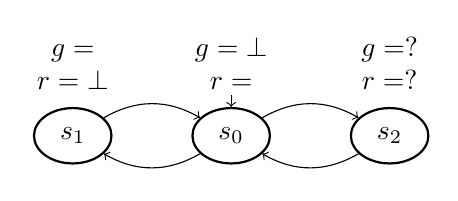
\begin{tikzpicture}[scale=0.33] %[x={10.0pt},y={10.0pt}]

\node [state, initial, initial text={},initial where=above](s_0)
[label={
[align=center,yshift=0.1cm]
%above:
% \includegraphics[width=50pt]{images/Red.pdf}
%$\boldsymbol{\overline{green}=T}$\\
$g=\color{black}\bot$\\
$r=\LTLtrue$
}] 
{$s_0$};   


\node[state] (s_1) 
[left=of s_0,
label={
[align=center,yshift=0.1cm]
%above:
% \includegraphics[width=50pt]{images/Green.pdf}
%$\boldsymbol{\overline{green}=F}$\\
$g=\color{black}\LTLtrue$\\
$r=\bot$
}]  
{$s_1$};

\node[state] (s_2) 
[right=of s_0,
label={
[align=center,yshift=0.1cm]
%above:
% \includegraphics[width=50pt]{images/Bo.pdf}
%$\boldsymbol{\overline{green}=\bot}$\\
$g=\color{black}?$\\
$r=?$
}]  
{$s_2$};


\path[->]      
(s_0) edge [bend left] node [above]{} (s_1) 
(s_1) edge [bend left] node [above]{} (s_0)
(s_0) edge [bend left] node [above]{} (s_2)
(s_2) edge [bend left] node [above]{} (s_0);   

\end{tikzpicture}
\caption{System model $M$}
\label{fig:modelmot}
\end{figure}


Regardless of the temporary incompleteness, the designer wants to evaluate the satisfaction of the properties of  interest. 
By model checking, it is possible to verify that the model does not contain any behavior that violates or possibly violates $\phi_1$. 
However, the result does not provide any information on why $\phi_1$ is satisfied.
Instead, a model checker equipped with a deductive verification framework would reveal that the system enters infinitely often state $s_0$, in which the red light is turned on, thus explaining why property $\phi_1$ is satisfied.

Let us now consider property $\phi_2$, which possibly holds.
The model checking algorithm returns a \emph{possible} counterexample: by turning off the green light in state $s_2$, the system may infinitely loop over $s_0$ and $s_2$ without $g$ ever being true. 
However, the search of a \emph{definitive} counterexample has failed.
The deductive verification framework would explain to the designer why this search failed.
As a matter of fact, if a counterexample is present, it must be present in any possible completion  of the model, i.e., for any possible assignment to the light in the state $s_2$.
But, let us consider a possible refinement of the incomplete state $s_2$ where the green light is on.
Since the green light is on in $s_1$ ($s_2$), it is possible to deduce that the light is eventually green in state $s_1$ ($s_2$).
Since it is allowed to loop over states $s_0$, $s_1$ and $s_2$, it is possible to deduce that ``always eventually green" is true in $s_0$, $s_1$ and $s_2$.
Thus, $\phi_2$ is satisfied in $s_0$, the initial state.
In conclusion, when the model checker returns maybe, it outputs a possible counterexample for a possible refinement of the incomplete states. 
In addition, the deductive verification framework would explain that the search of a definitive counterexample has failed in the case in which the green light is on in $s_2$.
This provides a useful insight to the designer, explaining that, by setting $g$ to $\LTLtrue$ in $s_2$, one obtains a model satisfying $\phi_2$ while, in the opposite case, $\phi_2$ is violated.


Finally, when property $\phi_3$ is considered, the model checking algorithm returns a definitive counterexample since $\phi_3$ is not satisfied, regardless of further refinements of $s_2$. Indeed, there exists an infinite run among states $s_0$ and $s_1$ in which a red light is not followed by a permanently green light. Indeed, the requirement that the designer probably meant to specify is $\LTLglobally (red \LTLimplication \LTLnext green)$.



%
%The model checker returns an ``unknown'' answer because if, in a future implementation, the semaphore is green in $s_2$, then the property holds. On the contrary, should not the green light be configured in $s_2$, the property would be violated.
%
%What our proposed approach offers is the ability to jointly analyze both potentially bad designs and potentially good designs.
%Especially in those cases where the model checker answer is ``unknown'', the designer is provided with information that can reveal itself fundamental to complete the current design. Namely: he/she obtains a counterexample that shows one violating behavior along with a proof that justifies why the current implementation of the model does not violate the property.
%The counterexample returned corresponds to the scenario in which the system infinitely loops over states $s_0$ and $s_2$.
%The provided proof explains  to the designer \emph{why} the search of a violating behavior has failed.
%This procedure considers a version of $M$ in which the $?$ values are substituted with $\LTLtrue$.
%It first identifies a set of axioms that specify why the search fails in some states of the model.
%By using a set of deductive verification rules it shows how these axioms imply the overall satisfaction of $\phi_3$.
%In this example, we first state what axiomatically holds in the states $s_1$ and $s_2$, which are the peripheral areas of the model.
%Since $s_1$ and $s_2$ are successors of $s_0$ we can inductively deduce what is satisfied in $s_0$. The final result, is reached by conjucting all the conclusiones gathered on the single model states.
%

%%%%


\section{Background}
\label{sec:preliminaries}
This section presents the modeling formalisms, their properties and verification algorithms upon which \NAME\ is based. It first briefly overviews how functional properties are checked over complete models.
Then it discusses how incomplete models are verified.
Finally, it describes how the deductive verification framework exploits the model checking procedure of complete models to generate a proof that explains why a property is satisfied.
An extended version of the paper, that includes all the formal details, can be found at \url{goo.gl/g3tmzG}.


\subsection{Checking complete models.}
%\textbf{Checking complete models.}
\label{sec:mcComplete}
Given a Kripke Structure $M$ (KS)~\cite{Kripke1963-KRISCO}, the model checking procedure verifies whether a Linear Temporal Logic (LTL)~\cite{pnueli1977temporal} formula $\phi$ holds or does not hold in $M$. 
The procedure works in three steps~\cite{clarke1999model}:
\begin{enumerate*}
\item generation of a non-deterministic B{\"u}chi automaton $\mathcal{A}_{\lnot\phi}$ from an LTL formula $\phi$;
\item generation of the product $\mathcal{G}=M \otimes\mathcal{A}_{\lnot\phi}$;
\item emptiness check of $\mathcal{G}$.
\end{enumerate*}




\subsection{Checking incomplete models.}
%\textbf{Checking incomplete models.}
\label{sec:mcIncomplete}
We present Partial Kripke Structures~\cite{bruns1999model} (PKSs), which is the formalism we assume the designer has used to describe the system under development.
We discuss the three-valued~\cite{bruns1999model} and thorough~\cite{bruns2000model} semantics of LTL formulae over PKSs, since the knowledge of these two semantics is necessary to understand when \NAME\ can be applied.
Finally, we introduce the verification procedure of an LTL formula over a PKS for the three-valued semantics, which is the base block upon which our deductive verification procedure is constructed.


\emph{Partial Kripke Structures} (PKSs) extend KSs by allowing a proposition in a given state to be labelled with $?$ to represent an unknown value of a proposition. 

\begin{definition}[Partial Kripke Structure \cite{bruns1999model} (PKS)]
A PKS $M$ is a tuple $\langle S, R, S_0,$ $ AP, L \rangle$,
where:
\begin{enumerate*}
\item[] $S$ is a set of \emph{states};
\item[] $R\subseteq S\times S$ is a \emph{left-total} \emph{transition relation} on $S$;
\item[] $S_0$ is a set of initial states;
\item[] $AP$ is a set of atomic propositions;
\item[] $L: S\times AP\rightarrow \{\top,?,\bot\}$ is a \emph{function} that, for each state in $S$, associates a truth value in the set $\{\top,?,\bot\}$ to every atomic proposition in $AP$.
\end{enumerate*}  
\end{definition}

The grade crossing semaphore, shown in Figure~\ref{fig:modelmot} and described in Section~\ref{sec:motivating}, is an example of how the system can be represented by means of a PKS.

A \emph{completion} of a PKS $M$ is a KS $M^\prime$ that completes $M$ by assigning values to the unknown propositions.
We will use $\mathcal{C}(M)$ to indicate all the completions of a PKS $M$.


Two different semantics of LTL can be considered: the three-valued or the thorough semantics.

%----------------------------------------------------------------------------------------------------------------------------------------------------------------
% Three-valued LTL semantic
%----------------------------------------------------------------------------------------------------------------------------------------------------------------
The \emph{three-valued LTL semantics} specifies that a formula $\phi$ definitely holds in a PKS $M$ if it is true for all possible values of the unknown propositions in $M$. 
Likewise, it is definitely violated if it is false despite the unknown values.
%A formula $\phi$ is not satisfied if there is a path $\pi$ in the PKS which violates $\phi$ despite the unknown values of the atomic propositions associated to the states of $\pi$.
%Otherwise the formula is unknown.

\begin{definition}[Three-valued LTL semantics~\cite{godefroid2011ltl}]
Given a PKS $M = \langle S, R,$ $S_0, AP, L \rangle$, a path $\pi=s_0,s_1,\ldots$, and a formula $\phi$, the three-valued semantics $[(M,\pi)\models\phi]$ is defined inductively as follows:
\begin{align*}
&[(M,\pi) \models p] & \buildrel \text{def}\over = &&& L(s_0,p)\\
&[(M,\pi) \models \lnot\phi] & \buildrel \text{def}\over = &&& \textnormal{comp}([(M,\pi) \models\phi]) \\
&[(M,\pi) \models \phi_1 \LTLand \phi_2] & \buildrel \text{def}\over =   &&& \min([(M,\pi) \models\phi_1],[(M,\pi) \models\phi_2])\\
&[(M,\pi) \models \LTLnext \phi] & \buildrel \text{def}\over =  &&& [(M,\pi^1) \models\phi]\\
&[(M,\pi) \models \phi_1 \LTLuntil \phi_2] & \buildrel \text{def}\over =  &&& \max_{j\geq 0}(\min(\{[(M,\pi^i) \models\phi_1]|i<j\} \cup \{[(M,\pi^j) \models\phi_2]\}))
\end{align*}
\end{definition}


The conjunction (disjunction) is defined as the minimum (maximum) of its arguments, following the order $\bot<?<\top$. Negation is defined by the function comp (complement), which maps $\top$ to $\bot$, $\bot$ to $\top$, and $?$ to $?$. These functions are extended to sets considering min($\emptyset$)=$\top$ and max($\emptyset$)=$\bot$.

Given a PKS $M = \langle S, R,$ $S_0, AP, L \rangle$, a state $s$, and a formula $\phi$,  $[(M, s) \models \phi] \buildrel \text{def}\over =   \min(\{[(M, \pi) \models \phi] \mid \pi^0=s\})$.
Intuitively this means that, given a formula $\phi$, each state $s$ of $M$ is associated with the minimum of the values obtained considering the LTL semantics over any path $\pi$ that starts in $s$.



%&[(M,\pi) \models \phi_1 \LTLuntil \phi_2] & = &&& max(\{min(\{[(M,\pi^i) \models\phi_1]|i<j\} \cup \{[(M,\pi^j) \models\phi_2]\})|j\geq 0\})\\


A PKS $M$ \emph{definitely satisfies} a property $\phi$ ($[M \models \phi]=\top$) iff for all initial states $s_0 \in S_0$ of $M$, $[(M, s_0) \models \phi]=\top$. 
A PKS $M$ \emph{does not satisfy} the property $\phi$ ($[M \models \phi]=\bot$) iff there exists an initial state $s_0 \in S_0$ of $M$ such that  $[(M, s_0) \models \phi]=\bot$.
A PKS \emph{possibly satisfies} $\phi$ otherwise.
In the rest of the paper we will use interchangeably the expressions ``$M$ definitely satisfies $\phi$'' and ``$\phi$ holds in $M$'', ``$M$ does not satisfy $\phi$'' and ``$\phi$ does not hold in $M$'', as well as ``$M$ possibly satisfies $\phi$'' and ``$\phi$ possibly holds in $M$''.



The three-valued semantics does not behave always as expected: there are cases in which $\phi$ possibly holds but all the KSs completions (obtained by replacing the $?$ values with $\top$ and $\bot$) actually satisfy (or do not satisfy)  $\phi$.
For instance, this happens when $\phi$ is a tautology or it is unsatisfiable with a traditional two-valued interpretation. 

The \emph{thorough LTL semantics}---differently from the three-valued semantics---specifies that a formula is possibly satisfied only if there exist two completion KSs $M_1$ and $M_2$, that definitely satisfy and violate $\phi$, respectively.

%DELETED
%Let the \emph{completions} $\mathcal{C}(M)$ of a PKS $M$ be the set of all the complete KS. Every,  KS $M_i \in \mathcal{C}(M)$ is such that, for each state, to every atomic proposition with value $?$ either the value $\top$ or $\bot$ is assigned.

\begin{definition}[Thorough semantics~\cite{bruns2000model}]
\label{def:thoroughsemantics}
Let $\phi$ be an LTL formula and $M$ a PKS, the truth value of a formula $\phi$ of a thorough temporal logic semantics, written $[M\models\phi]_t$, is defined as follows:

\begin{equation}
 [M \models\phi]_t \buildrel \text{def}\over = 
                						\begin{cases}
                  								\top & \quad  \text{if}\ M^\prime \models \phi \text{ for all } M^\prime \in \mathcal{C}(M)\\
                  								\bot & \quad  \text{if}\ M^\prime \not\models\phi \text{ for all } M^\prime \in \mathcal{C}(M)\\
                  								? &  \quad  \text{otherwise}
                							  \end{cases}      					  		   
\end{equation}

\end{definition}

\begin{proposition}[\cite{godefroid2011ltl}] 
\label{def:mcImpliesGmc}
Given a PKS and an LTL formula $\phi$,
\begin{enumerate}
\item $[M\models\phi] =$ $ \top \Rightarrow$ $ [M\models\phi]_t = \top$.
\item $[M\models\phi] = \bot \Rightarrow [M\models\phi]_t = \bot$.
\end{enumerate}
\end{proposition}
%
That is, a formula which is true (false) under the three-valued semantics is also true (false) under the thorough semantics.

Given the three-valued and the thorough semantics, there exists a subset of LTL formulae, indicated in literature as \emph{self-minimizing}, such that the two semantics coincide. Formally,

\begin{proposition}[\cite{godefroid2005MCvsGMC}]
\label{def:self-minimizing}
 Given a model $M$ and a  self-minimizing LTL property $\phi$, then $[M\models\phi]=[M\models\phi]_t$.
\end{proposition}
%In~\cite{godefroid2005MCvsGMC} the authors showed that many temporal-logic formulae of practical interest are self-minimizing.
%More precisely, all the formulae that do not contain atomic propositions with mixed polarity (negated and not negated) in their negation normal form are self-%minimizing; if the formulae follow specific patterns are self-minimizing;
%some LTL formulae that are not self-minimizing can be converted into self-minimizing LTL formulae using a procedure called semantic-minimization.
%The interested reader may refer to~\cite{godefroid2005MCvsGMC} for more details.
%
%

In the following, we present a model checking algorithm for LTL formulae when a three-valued semantics is considered. 
The algorithm exploits two classical model checking procedures for KSs.
These procedures consider a version of $M$, called \emph{complement-closed} structure~\cite{bruns2000model}, in which for every proposition $p \in AP$, there exists a new proposition $q$, called complement-closed proposition, such that $L(s,p)=$ comp$(L(s,q))$, for all $s \in S$.
The proposition $q$, whose value is complementary to the one of $p$, is indicated as $\overline{p}$.
For example, the complement-closed version of the PKS of the semaphore example is presented in Figure~\ref{fig:model}, where the atomic propositions $\overline{g}$ and $\overline{r}$ are associated with the complement of the values of  propositions green ($g$) and red ($r$), respectively.

\begin{figure}[t]
\begin{minipage}[b]{.5\textwidth}
  \begin{figure}[H]
 \centering
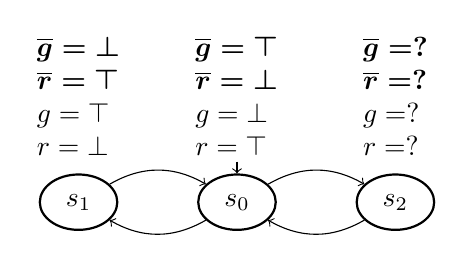
\begin{tikzpicture}[scale=0.33] %[x={10.0pt},y={10.0pt}]

\node [state, initial, initial text={},initial where=above](s_0)
[label={
[align=left,yshift=0.1cm]
above:
$\boldsymbol{\overline{g}=\top}$\\
$\boldsymbol{\overline{r}=\bot}$\\
$g=\color{black}\bot$\\
$r=\top$}] 
{$s_0$};   

\node[state] (s_1) 
[left=of s_0,
label={
[align=left,yshift=0.1cm]
above:
$\boldsymbol{\overline{g}=\bot}$\\
$\boldsymbol{\overline{r}=\top}$\\
$g=\color{black}\top$\\
$r=\bot$}]  
{$s_1$};

\node[state] (s_2) 
[right=of s_0,
label={
[align=left,yshift=0.1cm]
above:
$\boldsymbol{\overline{g}=?}$\\
$\boldsymbol{\overline{r}=?}$\\
$g=\color{black}?$\\
$r=?$}]  
{$s_2$};


\path[->]      
(s_0) edge [bend left] node [above]{} (s_1) 
(s_1) edge [bend left] node [above]{} (s_0)
(s_0) edge [bend left] node [above]{} (s_2)
(s_2) edge [bend left] node [above]{} (s_0);   

\end{tikzpicture}



\caption{The PKS of  the  crossing semaphore.}
\label{fig:model}
\end{figure}
\end{minipage}
\begin{minipage}[b]{.5\textwidth}
  \begin{figure}[H]
\centering
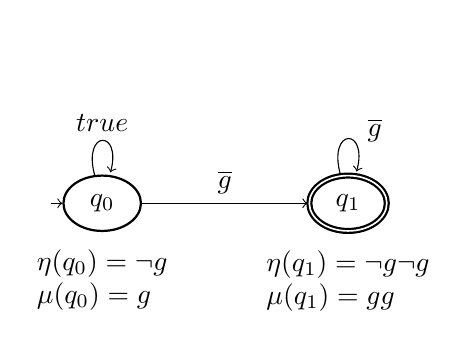
\begin{tikzpicture}[scale=0.33] %[x={10.0pt},y={10.0pt}]

\node[state, initial, initial text={}] (q_0) 
[label={
[align=left,yshift=-0.1cm]
below:
$\eta(q_0)= \LTLnext \LTLfinally \LTLglobally \lnot g$\\
$\mu(q_0)= \LTLnext \LTLglobally \LTLfinally g$}]
{$q_0$};
   
\node[state,accepting] (q_1) 
[right = 2.1cm of q_0,
label={
[align=left,yshift=-0.1cm]
below:
$\eta(q_1)= \lnot g \LTLand \LTLnext \LTLglobally \lnot g  $\\
$\mu(q_1)= g \LTLor \LTLnext \LTLfinally g$}]
{$q_1$};

\path[->]      
(q_0) edge [loop above]node [above]{$true$} (q_0) 
(q_0) edge node [above,align=center]
{\\ \\ \\ $\overline{g}$} (q_1)
(q_1) edge [loop above]node [above right, pos=0.8,align=center]
{\\ \\ \\ $\overline{g}$} (q_1);    

\end{tikzpicture} 
\caption{The BA associated with $\phi_2$.}
\label{fig:property}
\end{figure}
\end{minipage}
\end{figure}



%
%\begin{definition}[PKS optimistic and pessimistic labelling~\cite{bruns2000model}]
%Given a three-valued labelling function $L$,  we define the derived optimistic ($L_{opt}$) and pessimistic ($L_{pes}$) labelling function for every state s of the model $M$ as follows: 
%\begin{equation}
%    L_{opt}(s,p) \buildrel \text{def}\over = 
%                					\begin{cases}
%                  						\top & \quad  \text{if}\ L(s,p)=?\\
%                  						L(s,p) &  \quad otherwise
%                					\end{cases}
%\end{equation}            					  
%\begin{equation}      					  
%   L_{pes}(s,p) \buildrel \text{def}\over = 
%	                            \begin{cases}
%                  				       \bot  & \quad \text{if}\ L(s,p)=?\\
%                  						L(s,p) & \quad otherwise
%                					\end{cases}
%\end{equation}
%\end{definition}

The model checking procedure for a PKS $M$ is based on an optimistic and pessimistic approximation of $M$'s complement-closure.
The optimistic (pessimistic) approximation function $L_{opt}$  ($L_{pes}$) associates the value $\top$ ($\bot$) to each atomic proposition of the complement-closure of $M$ with value $?$.
Thus, in the optimistic (pessimistic) approximation, the propositions $g$ and $r$ associated with the value $?$ are assigned the value $\top$ ($\bot$).
Given a PKS $M=\langle S,R, S_0, L \rangle$, we have $M_{pes}=\langle S,R, S_0, L_{pes} \rangle$ for the pessimistic structure, and $M_{opt}=\langle S,R, S_0, L_{opt} \rangle$ for the optimistic one.
%
%The model checking procedure exploits the under and the over approximations as we show hereafter.

The three-valued model checking algorithm assumes that property $\phi$ is rewritten using complement-closed propositions. 
The rewriting procedure works in two steps.
First, the formula is expressed such that negations only appear in front of atomic propositions. 
Second, each negated proposition is substituted by the corresponding complemented proposition.


\begin{theorem}[Three-valued model checking~\cite{bruns2000model}\footnote{Note that Theorem~\ref{th:threevaluedMC} is stated for Positive Propositional Modal Logic in~\cite{bruns2000model} but is proved to be also valid for LTL (see \cite{bruns2000model,godefroid2005MCvsGMC,godefroid2011ltl}).}]
\label{th:threevaluedMC}
Let $\phi$ be an LTL formula obtained using the procedure just discussed, $M=\langle S, R, S_0, L\rangle $ a PKS with $s \in S$, and $M_{pes}$ and $M_{opt}$ the corresponding pessimistic and optimistic structures. Then
\begin{equation}
    [(M,s)\models\phi]  = 
                						 \begin{cases}
                  				 				\top & \quad \text{if}\ (M_{pes},s)\models\phi\\
                  								\bot & \quad \text{if}\ (M_{opt},s)\not\models\phi\\
                  								? & \quad  otherwise
                						\end{cases}
\end{equation}
\end{theorem}

This technique exploits two runs of the classical two-valued model checking performed respectively on a pessimistic and an optimistic completion of the incomplete model $M$.
Intuitively, in the construction of the optimistic completion $M_{opt}$, the algorithm ``tries to do its best" to build a KS which satisfies $\phi$. 
If a violating behavior is found in $M_{opt}$, then a definitive counterexample is returned since the property $\phi$ does not hold.
Vice versa, in the construction of the pessimistic completion $M_{pes}$, the three-valued model checker tries to construct a KS which violates $\phi$. 
If no violating behavior is found in $M_{pes}$, then $\phi$  definitely holds.
Otherwise, it could be the case where there exists some completion in which $\phi$ holds and others in which it does not hold. 
This implies that a $?$ value is returned by the three-valued model checker.
Note that whenever a $\top$ or $\bot$ value is returned, the property $\phi$ is guaranteed to be true/false in all the completions of $M$.
For additional details on this procedure see~\cite{bruns2000model,godefroid2011ltl}.




%\begin{theorem}(The verification procedure is correct)
%\end{theorem}
%\begin{proof}
%Given a self-minimizing temporal logic formula $\phi$, by Proposition~\ref{def:self-minimizing}, generalized (which is based on the thorough semantic) and
%three-valued model checking produce the same result.
%Thus, the considered three-valued model checking algorithm returns the correct value also under the thorough interpretation.
%\end{proof}


Properties $\phi_1$, $\phi_2$ and $\phi_3$ of the crossing semaphore example are respectively satisfied, possibly satisfied and not satisfied for the model $M$ of Figure~\ref{fig:model}.

Let us consider property $\phi_2$. The procedure first checks if $\phi_2$ is violated.
The intersection $I_{opt}$  between the optimistic structure $M_{opt}$ (obtained by changing all the $?$ values in $\LTLtrue$) and the BA $\mathcal{A}_{\neg\phi_2}$ associated with the property $\neg \phi_2$ (represented in Figure~\ref{fig:property}) is computed.
The automaton $I_{opt}$ is presented in Figure~\ref{fig:productOpt}.
The transitions marked with dashed-lines and the grey frames do not belong to the intersection: their meaning will be described in the following.
The state space of  $I_{opt}$ is explored in search of a definitive counterexample. 
Since in $I_{opt}$ no state labelled with an accepting state of  $\mathcal{A}_{\lnot\phi_2}$ (i.e., $\{q_1\}$) can be entered infinitely often, no counterexample is identified.
Then, the procedure checks if $\phi_2$ is possibly violated.
The intersection $I_{pes}$ between the pessimistic structure $M_{pes}$ (obtained by changing all the $?$ values in $\LTLfalse$) and $\mathcal{A}_{\neg\phi_2}$ is computed.
The automaton $I_{pes}$ is presented in Figure~\ref{fig:productPess}.
The state space of  $I_{pes}$ is explored in search of a possibly violating behavior.
Since it exists a state labelled with an accepting state of  $\mathcal{A}_{\lnot\phi_2}$ (i.e., $\{q_1\}$) which can be entered infinitely often (both $\langle s_2, q_1\rangle$ and $\langle s_0, q_1\rangle$), a possible counterexample is returned. 
Consequently, $\phi_2$ is possibly satisfied, i.e., there exists a completion $M_{pes}$ of $M$ that violates $\phi_2$.
For example, if $g=\bot$ and  $r=\bot$ to the propositions in $s_2$, we obtain a violating behavior when the system moves alternatively between $s_0$ and $s_2$. 




\begin{figure}[t]
\begin{minipage}[b]{.5\textwidth}
  \begin{figure}[H]
\centering




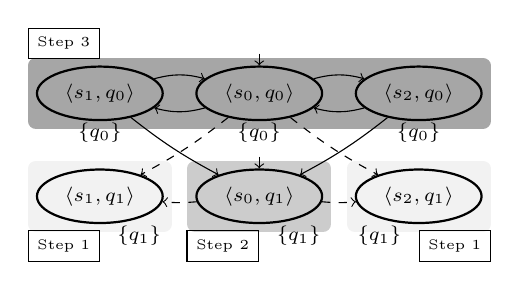
\begin{tikzpicture}[scale=0.33] %[x={10.0pt},y={10.0pt}]

\node[statep, initial, initial text={}, initial where=above] (s0q0) 
[label={[yshift=-1.1cm,xshift=0cm]\scriptsize $\{q_0\}$},font=\scriptsize] {$\langle s_0,q_0\rangle$}; 
\node[statep,  initial, initial text={}, initial where=above] (s0q1) 
[below = 0.6cm of s0q0,label={[yshift=-1.1cm,xshift=0.5cm]\scriptsize $\{q_1\}$},font=\scriptsize] {$\langle s_0,q_1\rangle$}; 

\node[statep] (s1q0) 
[left = 0.4cm of s0q0,label={[yshift=-1.1cm,xshift=0cm]\scriptsize $\{q_0\}$},font=\scriptsize] {$\langle s_1,q_0\rangle$}; 
\node[statep] (s1q1) 
[below = 0.6cm of s1q0,label={[yshift=-1.1cm,xshift=0.5cm]\scriptsize $\{q_1\}$},font=\scriptsize] {$\langle s_1,q_1\rangle$}; 

\node[statep] (s2q0) 
[right = 0.4cm of s0q0,label={[yshift=-1.1cm,xshift=0cm]\scriptsize $\{q_0\}$},font=\scriptsize] {$\langle s_2,q_0\rangle$}; 
\node[statep] (s2q1) 
[below = 0.6cm of s2q0,label={[yshift=-1.1cm,xshift=-0.5cm]\scriptsize $\{q_1\}$},font=\scriptsize] {$\langle s_2,q_1\rangle$}; 

%%LABELS for steps
\node[empty] (step3u) [above = 0.155cm of s0q0] {}; 
\node[empty] (step1u) [below = 0.155cm of s0q1] {}; 
\node[emptynode] (step3) [left = 1.9cm of step3u] {\tiny Step 3}; 
\node[emptynode] (step1) [left = 1.9cm of step1u] {\tiny Step 1}; 
\node[emptynode] (step1b) [right = 1.9cm of step1u] {\tiny Step 1}; 
\node[emptynode] (step2) [right= 1.1cm of step1] {\tiny Step 2};


\path[->]      
(s0q0) edge [bend left=15] node []{} (s1q0) 
(s1q0) edge [bend left=15] node []{} (s0q0)  

(s0q0) edge [bend left=15] node []{} (s2q0) 
(s2q0) edge [bend left=15] node []{} (s0q0)  

(s1q0) edge [bend right=5] node []{} (s0q1)
(s2q0) edge [bend left=5] node []{} (s0q1)

(s0q0) edge [bend left=5,dashed] node []{} (s1q1)
(s0q0) edge [bend right=5,dashed] node []{} (s2q1)

(s0q1) edge [bend left=5,dashed] node []{} (s1q1) 
(s0q1) edge [bend right=5,dashed] node []{} (s2q1) 
;    

\begin{pgfonlayer}{background}

%FAILED
\filldraw [line width=2mm,join=round,black!5]
(s1q1.south -| s1q1.west) rectangle (s1q1.north -| s1q1.east);
\filldraw [line width=2mm,join=round,black!5]
(s2q1.south -| s2q1.west) rectangle (s2q1.north -| s2q1.east);

%SUCCESSORS
\filldraw [line width=2mm,join=round,black!20]
(s0q1.south -| s0q1.west) rectangle (s0q1.north -| s0q1.east);

%INDUCTION
\filldraw [line width=2mm,join=round,black!35]
(s1q0.south -| s1q0.west) rectangle (s2q0.north -| s2q0.east);

\end{pgfonlayer}


\end{tikzpicture}

\caption{Product $I_{opt}=M_{opt}\otimes\mathcal{A}_{\lnot\phi_2}$}
\label{fig:productOpt}
 \end{figure}
\end{minipage}%
\begin{minipage}[b]{.5\textwidth}
  \begin{figure}[H]
\centering
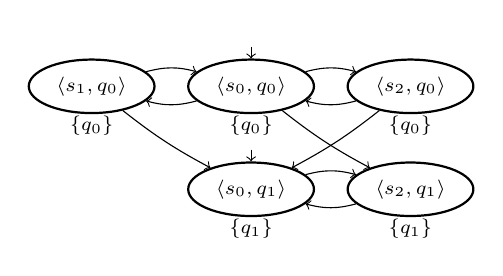
\begin{tikzpicture}[scale=0.33] %[x={10.0pt},y={10.0pt}]

\node[statep, initial, initial text={}, initial where=above] (s0q0) 
[label={[yshift=-1.1cm,xshift=0cm]\scriptsize $\{q_0\}$},font=\scriptsize] 
{$\langle s_0,q_0\rangle$}; 
\node[statep,  initial, initial text={}, initial where=above] (s0q1) 
[below = 0.6cm of s0q0,label={[yshift=-1.1cm,xshift=0cm]\scriptsize $\{q_1\}$},font=\scriptsize] {$\langle s_0,q_1\rangle$}; 

\node[statep] (s1q0) 
[left = 0.4cm of s0q0,label={[yshift=-1.1cm,xshift=0cm]\scriptsize $\{q_0\}$},font=\scriptsize] {$\langle s_1,q_0\rangle$}; 
%\node[statep] (s1q1) [right = 1.2cm of s1q0,label={[yshift=-1.1cm]\small $\{q_1\}$},font=\scriptsize] {$\langle s_1,q_1\rangle$}; 

\node[statep] (s2q0) [right = 0.4cm of s0q0,label={[yshift=-1.1cm,xshift=0cm]\scriptsize $\{q_0\}$},font=\scriptsize] {$\langle s_2,q_0\rangle$}; 
\node[statep] (s2q1) [below = 0.6cm of s2q0,label={[yshift=-1.1cm,xshift=0cm]\scriptsize $\{q_1\}$},font=\scriptsize] {$\langle s_2,q_1\rangle$}; 

\path[->]      
(s0q0) edge [bend left=15] node []{} (s1q0) 
(s1q0) edge [bend left=15] node []{} (s0q0)  

(s0q0) edge [bend left=15] node []{} (s2q0) 
(s2q0) edge [bend left=15] node []{} (s0q0)  

(s1q0) edge [bend right=5] node []{} (s0q1)
(s2q0) edge [bend left=5] node []{} (s0q1)

%(s0q0) edge [bend left=5,dashed] node []{} (s1q1)
(s0q0) edge [bend right=5] node []{} (s2q1)

%(s0q1) edge [bend left=5,dashed] node []{} (s1q1) 
(s0q1) edge [bend left=15] node []{} (s2q1) 
(s2q1) edge [bend left=15] node []{} (s0q1) 
;    

\end{tikzpicture} % pic 1
\caption{Product $I_{pes}=M_{pes}\otimes\mathcal{A}_{\lnot\phi_2}$}
\label{fig:productPess}
 \end{figure}
\end{minipage}%
\end{figure}

\subsection{Deductive verification}
%\textbf{Constructing a Temporal Logic Proof.}
\label{sec:theoremProving}
The deductive verification framework used in this work is based on~\cite{peled2001model}.
It is developed on top of the two-valued model checker described in Section~\ref{sec:mcComplete}.
Given a structure $M$ and an LTL property $\phi$, which is satisfied by $M$, the deductive verification framework produces a proof which explains why $M \models \phi$.
The algorithm considers the intersection automaton $\mathcal{G}=M\otimes\mathcal{A}_{\lnot\phi}$.

The approach described in the following is built on three elements.
\begin{enumerate*}
\item every state $q\in Q$ of $\mathcal{A}_{\lnot\phi}$ is associated with an LTL formula $\eta(q)$ such that, for every accepting run $\sigma=q_0,q_1,...$ of $\mathcal{G}$, $\sigma_i\models\eta(q_i)$. This formula is computed during the procedure that converts the LTL formula $\neg \phi$ into $\mathcal{A}_{\lnot\phi}$~\cite{gerth1996ltl2ba}. For instance, the state $q_1$ of the automaton presented in Figure~\ref{fig:property} is associated with the formula $\eta(q_1)= \lnot g \LTLand \LTLnext \LTLglobally \lnot g$;
\item given a state $\langle s, q \rangle$ of the automaton $M\otimes\mathcal{A}_{\lnot\phi}$, the property $\eta(q)$ associated with the state $q$ of $\mathcal{A}_{\lnot\phi}$ is \emph{not} satisfied in $s$. 
Indeed, if $\eta(q)$ was satisfied, a counterexample would be found.
Thus, the negation $\mu(q)$ of $\eta(q)$ holds in $s$;
\item each node $\langle s, q \rangle$  which was not created during the computation of $M\otimes\mathcal{A}_{\lnot\phi}$, is such that $s$ does not satisfy $\eta(q)$, i.e., $s \models \mu(q)$.
Each of these nodes, called \emph{failed node}, causes a failure in the search of a counterexample and ensures the satisfaction of $\phi$ in the corresponding state of the system.
\end{enumerate*}

The deductive verification framework first enriches the product automaton $M\otimes\mathcal{A}_{\lnot\phi}$ by considering also failed nodes as part of it.
Each failed node is a node in which the search of a counterexample has failed. 
Thus,  given a failed node $\langle t,p \rangle$,  we can write the failure axiom $t\models \mu(p)$.
For example, the node $\langle s_1, q_1 \rangle$ of the intersection automaton presented in Figure~\ref{fig:productOpt} is a failed node since $s_1$ satisfies the property $\mu(q_1)= g \LTLor \LTLnext \LTLfinally g$ associated with the state $q_1$.

Then, a set of deductive rules is applied to produce the proof, specifically:
\begin{enumerate*}
\item \emph{Successors rule.} Given a state $\langle s, q\rangle$ of the intersection automaton, if for each of its successors $\langle s_i, q_j\rangle$ the state $s_i$ of $M$ satisfies the formula $\mu(q_j)$, then also $s$ satisfies $\mu(q)$.
Intuitively, the rule is based on two observations.
First, each successor  $\langle s_i, q_j\rangle$ of  $\langle s, q\rangle$ does not cause a violation of $\phi$, i.e., it ensures that $s_i \models \mu(q_j)$.
Second, by moving from $\langle s, q\rangle$ to $\langle s_i, q_j\rangle$ the system has not violated the property of interest, since no counterexample was found.
Thus, it must be that $s$ satisfies $\mu(q)$.
\item \emph{Induction rule.} It is a generalization of the successors rule applied on strongly connected components (SCCs). 
Given a strongly connected component $\mathcal{X}$, let us identify with $Exit(\mathcal{X})$ the set of all nodes $\langle s_i, q_j\rangle$ that do not belong to $\mathcal{X}$ and have an incoming transition from a source node in $\mathcal{X}$.
If every node $\langle s_i, q_j\rangle \in Exit(\mathcal{X})$ is such that $s_i \models \mu(q_j)$, we can conclude that, for every node $\langle s, q \rangle \in \mathcal{X}$, $s \models \mu(q)$ holds.
Intuitively, since all the ``successors'' of $\mathcal{X}$ (the nodes in $Exit(\mathcal{X})$) ensure the property satisfaction and the states in $\mathcal{X}$ do not violate the property of interest (no counterexample has been found in the intersection automaton), it must be that each state $s$ satisfies the corresponding property $\mu(q)$. 
\item \emph{Conjunction rule.} It allows connecting any pair of conclusions made on a given state and making temporal logic interferences. 
All the formulae computed for a given state $s$ are and-combined.
\end{enumerate*}

These rules are applied considering the partial ordering relation $\prec$ between SCCs. 
The relation $\mathcal{X} \prec \mathcal{X}'$ holds if there exists a transition from some state in $\mathcal{X}$ to some state in $\mathcal{X}'$. 
If $\mathcal{X} \prec \mathcal{X}'$, before considering the component  $\mathcal{X}$, it is necessary to compute the proof of $\mathcal{X}'$.

Additional details can be found in the extended version of this paper.

%The deductive verification procedure presented in this section modifies the one proposed in~\cite{peled2001model} by identifying the failed nodes as defined in Formula~\ref{eq:failedTransition}. 
%Furthermore, it does not consider fairness conditions in the induction rule.
%For additional details, the interested reader may refer to~\cite{peled2001model}.

\section{\NAME}
\label{sec:contribution}
\input{sections/Contribution.tex}

%\label{sec:example}
%



















\section{Preliminary evaluation}
\label{sec:preliminaryEvaluation}
This section discusses how \NAME\ supports the designer in the development of the system that satisfies the properties of interest.
We first consider the example introduced in Section~\ref{sec:motivating} w.r.t. property $\phi_2$. Then, properties $\phi_1$ and $\phi_3$ are also briefly discussed.


\textbf{Property $\boldsymbol{\phi_2}$.} 
The property $\phi_2=\LTLglobally \LTLfinally green$ specifies that green lights up infinitely often.
Even if in state $s_1$ the green light is on, the property is ``only" possibly satisfied.
\NAME\ returns the possible counterexample $(s_0, s_2)^\omega$, that shows why $\phi_2$ is possibly satisfied.
Specifically,  by looping an infinite number of time on states $s_0$ and $s_2$ the green light will not be turned on.
This is a possible counterexample since the value of the $green$ proposition in $s_2$ is currently unspecified.
Since the property $\phi_2$ is possibly satisfied, the search of a definitive counterexample has failed.
\NAME\ computes a proof that explains the motivation.
To search for a counterexample, the intersection automaton $M_{opt}$ presented in Figure~\ref{fig:productOpt} is explored by \NAME\ during the proof computation. The obtained proof is presented in Table~\ref{table:proof}, where $g$ stands for $green$.
The nodes that have been analyzed in different steps are circled  in Figure~\ref{fig:productOpt} through different grey frames.
(\emph{Step1}). \NAME\ analyzes the failed nodes, i.e., the nodes in the set $Fail(I_{opt})$.
Since in these nodes the search for a counterexample trivially fails, the formula associated with the corresponding states of $\mathcal{A}_{\lnot\phi_2}$ holds.
Thus, since the state $\langle s_1, q_1 \rangle$ of the intersection automaton is a failed node, the formula $green \LTLor \LTLnext \LTLfinally green$ (valid in $q_1$) is satisfied by the model state $s_1$.
This formula is effectively true in $s_1$ since the green light is on.
By means of a similar reasoning, the algorithm states that the property  $green \LTLor \LTLnext \LTLfinally green$ also holds in $s_2$. Indeed, since in the optimistic model the green light is on in $s_2$, the search of a counterexample has failed in $\langle s_2, q_1 \rangle$.
(\emph{Step2}). Since all the successors of $\langle s_0, q_1 \rangle$ satisfy $green \LTLor \LTLnext \LTLfinally green$, it is possible to deduce that this property is also satisfied in $s_0$.
(\emph{Step3}). The induction rule is applied considering the strongly connected component  $\left \{ \langle s_0, q_0 \rangle, \langle s_1, q_0 \rangle, \langle s_2, q_0 \rangle \right \}$.
The rule allows to conclude that $s_0$ satisfies the property $\LTLnext \LTLglobally \LTLfinally green$.
(\emph{Step4}). \NAME\ applies the conjunction rule to $s_0$.
Since $s_0$ satisfies both $\LTLnext \LTLglobally \LTLfinally green$ and $green \LTLor \LTLnext \LTLfinally green$, it is possibly to deduce that $s_0$ satisfies the property $\phi_2$.
This provides an interesting insight to the designer: if she/he does her/his ``best" to satisfy the property (she/he turns the green light on in $s_2$) the property becomes satisfied. The proof clearly states why.


\begin{table}[t]
\centering
\caption{Proof that $\phi_2$ is not violated.}
\label{table:proof}
\begin{tabular}[b]{ | p{1.8cm} | p{2.1cm} | p{4.3cm} | p{3cm} |  }
\hline
\emph{Step 1} &
\emph{Step 2} &
\emph{Step 3} &
\emph{Step 4}\\
\hline
%%\multicolumn{4}{|c|}{Steps}  \\
%% \hline
\textbf{Fail} & 
\textbf{Successors} &
\textbf{Induction} &
\textbf{Conjunction}\\
 \hline
 $\langle s_2,q_1\rangle,$\newline
$ \langle s_1,q_1\rangle$
 &
 $\langle s_0,q_1\rangle$ 
 &
 $\mathcal{X}=\{\langle s_0,q_0\rangle,\langle s_1,q_0\rangle,\langle s_2,q_0\rangle\}$
 $Exit(\mathcal{X})=\{\langle s_0,q_1\rangle,\langle s_1,q_1\rangle,$ $\langle s_2,q_1\rangle\}$
 &
The initial node $s_0$ \\	
 \hline
 \inferrule{s_1 \in Fail(I_{opt})\\
 s_2 \in Fail(I_{opt})
}{ s_1\models g \LTLor \LTLnext \LTLfinally g \\
 s_2\models g \LTLor \LTLnext \LTLfinally g}
  & 
\inferrule{s_0\rightarrow\{s_1,s_2\} \\
 s_1\models g \LTLor \LTLnext \LTLfinally g \\
  s_2\models g \LTLor \LTLnext \LTLfinally g }
 {s_0\models g \LTLor \LTLnext \LTLfinally g} 
  &
 \inferrule{ 
 s_0\models g \LTLor \LTLnext \LTLfinally g \\
  s_1\models g \LTLor \LTLnext \LTLfinally  g \\
  s_2\models g \LTLor \LTLnext \LTLfinally g \\
s_0\rightarrow \{s_1,s_2 \} \\\\
 s_1\rightarrow \{s_0 \} \\\\
 s_2\rightarrow \{s_0 \}   
   }
 {s_0\models \LTLnext \LTLglobally \LTLfinally g \\
 s_1\models \LTLnext \LTLglobally \LTLfinally g \\
 s_2\models \LTLnext \LTLglobally \LTLfinally g }
  &
\inferrule{
 s_0\models \LTLnext \LTLglobally \LTLfinally g \\
  s_0\models g \LTLor \LTLnext \LTLfinally g \\
 \LTLnext \LTLglobally \LTLfinally g \LTLand  (g \LTLor  \LTLnext \LTLfinally g)\rightarrow \phi_2 }
 {s_0\models \phi_2}  \\
\hline

\end{tabular}
\end{table}



\textbf{Property $\boldsymbol{\phi_1}$.}
The property $\phi_1=\LTLglobally \LTLfinally red$ specifies that red lights up infinitely often.
The designer wants to know whether the model of Figure~\ref{fig:modelmot} satisfies $\phi_1$.
Intuitively, it is sufficient to observe that the proposition $red$ is evaluated with $\LTLtrue$ in the state $s_0$ and that the system always returns to this state (after visiting either $s_1$ or $s_2$).
\NAME\ returns $\LTLtrue$ as its verification result and produces a proof that highlights how and why a definite counterexample is not found in the graph. First, it identifies the nodes $\langle s_0, q_1 \rangle$ and $\langle s_2, q_1 \rangle$ as failed. The conclusions found on these nodes are propagated to the node $\langle s_1, q_1 \rangle$. All the successors of the SCC formed by the intersection states related to the property state $q_0$ are analyzed. Therefore conclusions are drawn also on this SCC. 
The proof is not reported for brevity and it follows the same pattern as the one in Table~\ref{table:proof}.


\textbf{Property $\boldsymbol{\phi_3}$.}
$\LTLglobally (red \LTLimplication \LTLglobally green)$ cannot be satisfied by the chosen model. Therefore \NAME\ returns a definite counterexample, e.g. $(s_0, s_1)^\omega$.



\section{Discussion}
\label{sec:discussion}
This section elaborates on the applicability of \NAME. 

\emph{Three-valued vs thorough semantics.} As previously discussed, \NAME\ does not produce a useful result when a thorough semantics of LTL formulae is considered and a $?$ value is returned.
Indeed, the property could be $\LTLtrue$, $?$ or $\LTLfalse$ w.r.t. the thorough semantics.
The generalized model checking algorithm~\cite{bruns2000model}(which levies a performance penalty) could be used to discriminate between these cases.
In \cite{gurfinkel2005thorough}, the authors analyze how often this additional check really helps.
They show that whenever the model is built using predicate abstraction~\cite{graf1997construction}, the thorough check does not provide additional precision\footnote{The results of~\cite{gurfinkel2005thorough} are presented for CTL properties; however the authors specify that the results naturally extend to LTL.}.
It is also argued that in many practically interesting cases, the thorough semantics is not more precise than the three-valued one. 
For these reasons, \NAME\ can be usefully applied in most of the real world applications.

\emph{Temporal patterns of self-minimization.} 
\NAME\ always produces a correct result when the LTL formula is self-minimizing.
In~\cite{godefroid2005MCvsGMC} the authors propose a first grammar for this LTL subset. 
The grammar can be used by the designer to generate formulae that are (by construction) self-minimizing, or  to check whether a specific formula is self-minimizing, i.e., if the formula is compliant with the grammar, then it is self-minimizing.
The authors also argue that the set of self-minimizing LTL formulae contains most of the properties of practical interest, such as absence, universality, existence, response and response chain. 
The grammar presented in~\cite{godefroid2005MCvsGMC} is improved in~\cite{antonik2006efficient}, where the authors consider popular syntactic specification patterns, documented at a community-led pattern repository, and check whether the formulae that are compliant with these patterns are self-minimizing.
It is shown that many such patterns are self-minimizing and that, the ones that are not, can be transformed with linear blowup into a self-minimizing LTL formula.
Thus, in most cases, the designer will consider a formula that is self-minimizing. A syntactic check can be used to prove self-minimization before running \NAME .

\emph{Checking whether an LTL formula is self-minimizing.} Checking whether an LTL formula is self-minimizing (if it is not compliant with one of the syntactic patterns) is expensive, since it requires to compute an automaton that is exponential in $|\phi|$~\cite{godefroid2005MCvsGMC}. 
However, if $\phi$ satisfies some constraints (sufficient conditions) then it is self-minimizing.
For example, if it is in its negation normal form and no proposition occurs in mixed polarity, then $\phi$ is self-minimizing.
These checks can be implemented in \NAME . Note that, some LTL formulae can be transformed into their equivalent self-minimizing version, but not all the LTL formulae have a semantic minimization in LTL~\cite{godefroid2005MCvsGMC}.

\emph{Scalability.} Three-valued model checking is as expensive as classical model checking~\cite{bruns1999model}, which is commonly used to analyze real world problems~\cite{Woodcock:2009:FMP:1592434.1592436}.
Deductive verification has been employed successfully in the verification of digital hardware and software systems~\cite{rajan1995integration}.
However, there are inherent limits to the efficiency with which expressive general-purpose logics can be fully mechanized. 
Two approaches have been proposed in literature to overcome this limitation:
\begin{enumerate*}
\item  using interactive deductive verification tools so that correctness proofs can be developed through a combination of user guidance and limited forms of automated deduction;
\item considering useful fragments of logic that can be mechanized very effectively.
\end{enumerate*}
Since \NAME\ simply combines multi-valued model checking and theorem proving, its scalability improves  as the performance of the employed model checking and deductive verification  frameworks enhances.




\section{Related Work}
\label{sec:stateoftheart}
Three-valued~\cite{larsen1988modal,godefroid2001abstraction,bruns1999model,bruns2000model,benevs2009checking,godefroid2011ltl} and multi-valued~\cite{gurfinkel2003multi,bruns2004MCmultivalued} model checking techniques have been used to verify models that are incomplete, i.e., in which some information is missing. 
Two types of semantics are usually considered in these works: compositional (three-valued) and/or non-compositional (thorough).
The compositional semantics exploits the Kleene algebraic structure between the values $\{false, \bot, true \}$. 
The non-compositional semantics is  based on the completeness preorder.
These two semantics have been analyzed in many works, such as~\cite{gurfinkel2005thorough,godefroid2005MCvsGMC}.
Depending on the modeling formalism, different model checking techniques have been developed. For example, several works proposed in literature consider Partial Kripke Structures (e.g.,~\cite{bruns1999model,bruns2000model,godefroid2011ltl,gurfinkel2003multi,bruns2004MCmultivalued}), others Modal Transition Systems (e.g.,~\cite{larsen1988modal,godefroid2001abstraction}). 
However, to the best of our knowledge, none of these approaches has been combined with deductive verification.  

Deductive verification includes a set of techniques that establish the validity of the formula (for more information see~\cite{manna2012temporal}).
Some works have used deductive verification as a means to enrich the information returned by model checking~\cite{gurfinkel2003proof,clarke1995efficient}.
In other techniques~\cite{namjoshi2001certifying,cleaveland2002evidence,rajan1995integration}, the idea is to exploit the structure of the state space generated by the model checker to explain why a property holds.
To the best of our knowledge, none of these approaches has been applied in a multi-valued context.





\section{Conclusions}
\label{sec:conclusions}
We have proposed \NAME, a framework that enhances a three-valued model checker with a deductive verification engine. 
Whenever the property of interest is definitely satisfied, or possibly satisfied, \NAME\ provides the designer with additional information regarding why a certain result is returned by the model checker.
The proof gives intuition on what is working correctly in the current design and insights for the next development rounds.
The  presented framework can be implemented on top of existing model checking tools based on automata theory.

\NAME\ has been evaluated considering a simple semaphore example, which showed  the usefulness  of the approach.
We proved that the result generated by \NAME\ is always valid when self-minimizing LTL formulae are considered.
We discussed that self-minimizing formulae can be constructed following specific patterns and that checking whether an LTL formula is self-minimizing can be done using appropriate procedures.
We also argued that most of the properties of practical interest are already self-minimizing and that some LTL formulae can be transformed into a self-minimizing version.
We showed that when non self-minimizing LTL formulae are considered, \NAME\ produces a valid result in most of the cases: when a $\LTLtrue$ or $\LTLfalse$ value is returned, and also when a $?$ value is returned and the formula is possibly satisfied under the thorough semantics.
Finally, we pointed out that \NAME\ improves as model checking and deductive verification frameworks enhance. 

As future work, we aim to implement \NAME\ by integrating  existing model checking and theorem proving frameworks.
Additionally, we will prove the usefulness of \NAME\ over a real world example.

\bibliographystyle{abbrv}
\bibliography{sigproc} 


%\section*{Appendix:}


\end{document}
